% ============================================================
% Wide View and Line Filters for Edge Detection — Presentation
% ============================================================
% Compile with XeLaTeX:  xelatex main.tex && xelatex main.tex
% ============================================================

\documentclass[10pt, aspectratio=169]{beamer}

\usetheme{uofsc}
\usepackage{booktabs}
\usepackage{amsmath,amssymb}
\usepackage{hyperref}

% --- Presentation Metadata ---
\title[WVF/LF Edge Detection]{A Comprehensive Evaluation of Wide View and Line Filters for Edge Detection}
\subtitle{Parameter Optimization, Benchmarking, and Noise Robustness}
\author[J.C. Vaught]{J.C. Vaught\texorpdfstring{\\}{, }University of South Carolina}
\institute[UofSC]{}
\date{}

% ============================================================
\begin{document}

% ------ Title Slide ------
{
  \setbeamertemplate{footline}{}
  \begin{frame}[plain]
    \titlepage
  \end{frame}
}

% ------ Outline ------
\begin{frame}{Outline}
  \tableofcontents
\end{frame}

% ============================================================
\sectionsubtitle{The edge detection problem and motivation}
\section{Introduction}

\begin{frame}{The Edge Detection Landscape}
  Edge detection has evolved through three generations of methods.

  \begin{enumerate}
    \item \textbf{Classical operators} (Sobel, Prewitt, Canny): fixed-size kernels, simple but limited adaptability
    \item \textbf{Training-free extended filters} (WVF, LF): local polynomial fitting over large neighborhoods, no learned parameters
    \item \textbf{Deep learning} (DexiNed, TEED, PiDiNet, NBED, DiffusionEdge): learned edge representations, highest clean-data scores
  \end{enumerate}

  \vspace{0.5em}
  Bagan and Wang's Wide View Filter (WVF) and Line Filter (LF) sit between classical simplicity and DL complexity --- but are their published parameters optimal?
\end{frame}

\begin{frame}{Research Questions}
  This study addresses four questions through a comprehensive four-part investigation.

  \begin{enumerate}
    \item Are the published WVF/LF parameters ($N_p = 250$, $N_s = 18$, $d = 4$) optimal for standard benchmarks?
    \item How do optimally-tuned WVF/LF compare against 54 classical operators and 5 DL models?
    \item Does the WVF's extended spatial support provide noise robustness advantages over learned models?
    \item Are these findings statistically validated across datasets?
  \end{enumerate}

  \vspace{0.5em}
  Total scope: \textbf{500,000+} individual filter evaluations across 330 images and 4 datasets.
\end{frame}

% ============================================================
\sectionsubtitle{WVF and LF formulations}
\section{Methods}

\begin{frame}{Wide View Filter (WVF)}
  For a target pixel $\mathbf{p}$, the WVF selects $N_p$ nearest neighbors within a circular support. At each orientation $\theta_k$, it fits a polynomial of degree $d$ via least squares.

  \vspace{0.3em}
  The edge response is the maximum absolute normal derivative over all orientations:
  \[
    R_{\text{WVF}}(\mathbf{p}) = \max_{k = 1, \ldots, N_s} |\hat{c}_2^{(k)}|
  \]

  \vspace{0.3em}
  Three tunable parameters:
  \begin{itemize}
    \item $N_p$: support size (number of neighbor pixels)
    \item $N_s$: number of candidate orientations
    \item $d$: polynomial degree
  \end{itemize}
\end{frame}

\begin{frame}{Line Filter (LF)}
  The LF extends WVF by chaining $2m + 1$ WVF evaluations along a line at each orientation.

  \vspace{0.3em}
  Virtual expansion points are placed at:
  \[
    \mathbf{v}_j^{(k)} = \mathbf{p} + j(\cos\theta_k, \sin\theta_k), \quad j = -m, \ldots, m
  \]

  Derivative estimates are combined via Gaussian-weighted averaging:
  \[
    R_{\text{LF}}^{(k)}(\mathbf{p}) = \left| \sum_{j=-m}^{m} w_j \hat{c}_{2,j}^{(k)} \right|
  \]

  \vspace{0.3em}
  Additional parameter $m$ (line half-width) controls tangential averaging.
  At $m = 14$ (published), LF is $\sim$29$\times$ slower than WVF.
\end{frame}

\begin{frame}{Experimental Setup}
  \begin{table}
    \centering
    \caption{Datasets used in the evaluation (330 images total).}
    \begin{tabular}{lcl}
      \toprule
      \textbf{Dataset} & \textbf{Images} & \textbf{Resolution} \\
      \midrule
      UDED       & 30  & variable \\
      BIPED v1   & 50  & 1280 $\times$ 720 \\
      BIPED v2   & 50  & 1280 $\times$ 720 \\
      BSDS500    & 200 & 481 $\times$ 321 \\
      \bottomrule
    \end{tabular}
  \end{table}

  \vspace{0.3em}
  \begin{itemize}
    \item \textbf{WVF grid}: 1,206 valid configurations ($N_p \times N_s \times d$)
    \item \textbf{LF grid}: 168 configurations (adding $m$)
    \item \textbf{Classical baselines}: 54 configurations across 7 operator families
    \item \textbf{DL baselines}: DexiNed, TEED, PiDiNet, NBED, DiffusionEdge
  \end{itemize}
\end{frame}

% ============================================================
\sectionsubtitle{Published parameters are substantially suboptimal}
\section{Parameter Ablation}

\begin{frame}{WVF: Support Size Dominates Performance}
  \begin{columns}[T]
    \begin{column}{0.45\textwidth}
      Key findings from single-image ablation:
      \begin{enumerate}
        \item ODS peaks at $N_p = 30$--$50$, not 250
        \item $N_s$ saturates by 4--6 orientations
        \item $d = 2$ consistently outperforms $d = 4$
      \end{enumerate}

      \vspace{0.5em}
      At published $N_p = 250$: ODS $\approx$ 0.71 versus optimal 0.86 --- a 0.15 gap.
    \end{column}
    \begin{column}{0.52\textwidth}
      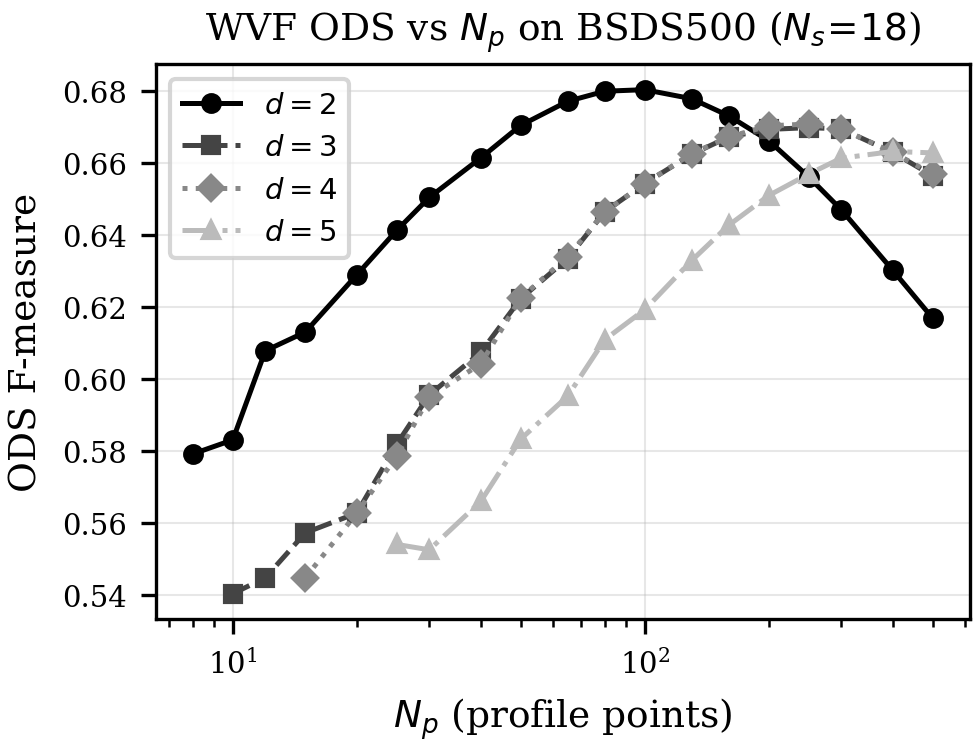
\includegraphics[width=\textwidth]{figures/fig_wvf_ods_vs_np.png}
    \end{column}
  \end{columns}
\end{frame}

\begin{frame}{Orientation Count Saturates Early}
  \begin{columns}[T]
    \begin{column}{0.45\textwidth}
      $N_s$ has minimal effect beyond 4--6 orientations.

      \vspace{0.5em}
      The difference between $N_s = 6$ and $N_s = 120$ is typically less than 0.005 ODS.

      \vspace{0.5em}
      Reducing $N_s$ from 18 to 4 yields a $4.5\times$ speedup with no loss in edge quality.
    \end{column}
    \begin{column}{0.52\textwidth}
      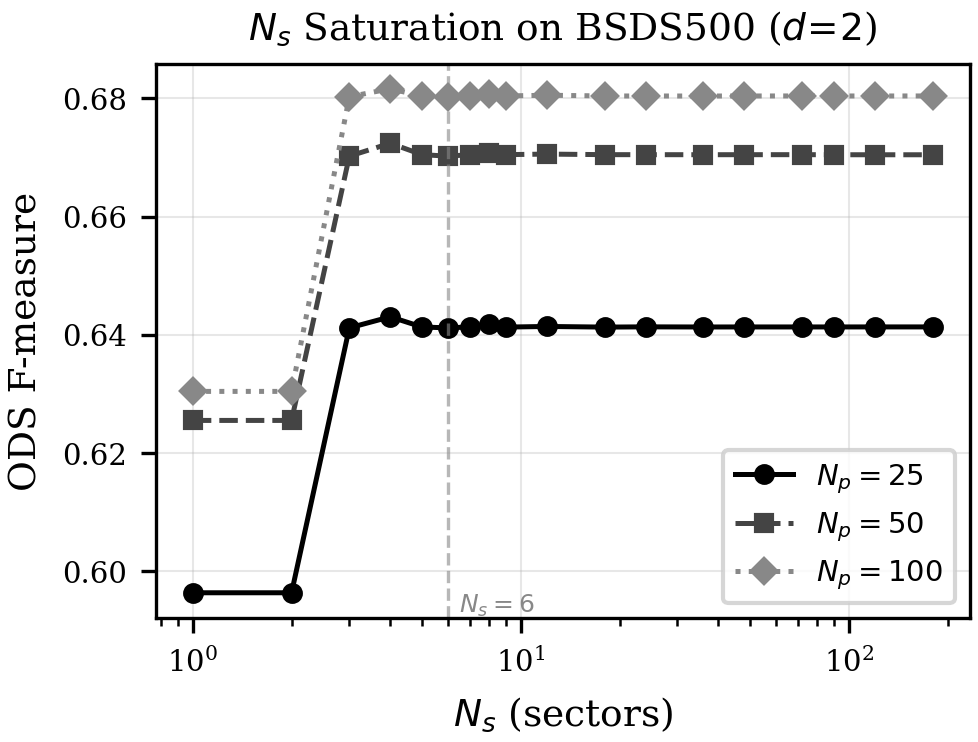
\includegraphics[width=\textwidth]{figures/fig_ns_saturation.png}
    \end{column}
  \end{columns}
\end{frame}

\begin{frame}{$N_p$ vs $N_s$ Heatmap}
  \begin{columns}[T]
    \begin{column}{0.35\textwidth}
      The dominant variation is along $N_p$.

      \vspace{0.5em}
      The optimal region forms a horizontal band at $N_p \approx 25$--$50$, largely invariant to $N_s$.

      \vspace{0.5em}
      This confirms: \textbf{support size is the critical parameter}.
    \end{column}
    \begin{column}{0.62\textwidth}
      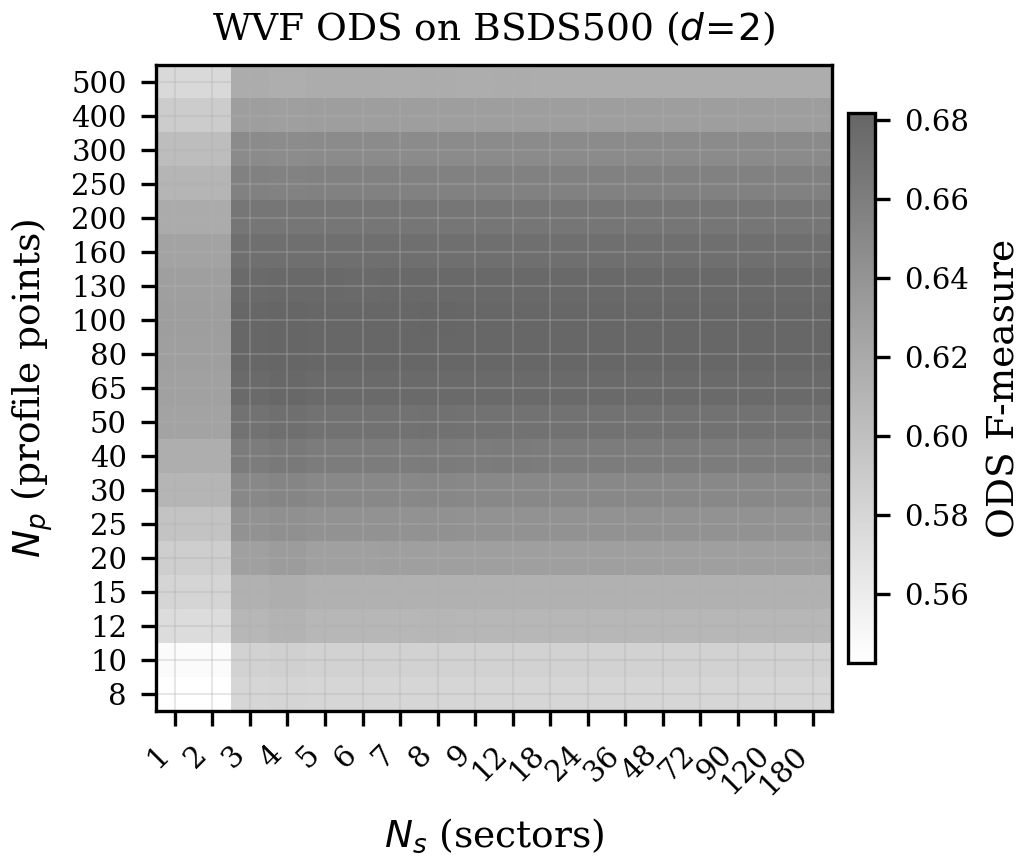
\includegraphics[width=\textwidth]{figures/fig_wvf_heatmap_np_ns.png}
    \end{column}
  \end{columns}
\end{frame}

\begin{frame}{Full-Dataset Results: Optimized vs. Published}
  \begin{table}
    \centering
    \caption{ODS improvement from parameter optimization across all datasets.}
    \begin{tabular}{lcccccc}
      \toprule
      \textbf{Dataset} & \textbf{Best WVF} & \textbf{Bagan WVF} & \textbf{$\Delta$} & \textbf{Best LF} & \textbf{Bagan LF} & \textbf{$\Delta$} \\
      \midrule
      UDED      & 0.899 & 0.847 & +0.052 & 0.887 & 0.729 & +0.158 \\
      BIPED v1  & 0.812 & 0.767 & +0.045 & 0.802 & 0.643 & +0.159 \\
      BIPED v2  & 0.830 & 0.783 & +0.047 & 0.819 & 0.658 & +0.161 \\
      BSDS500   & 0.682 & 0.671 & +0.011 & 0.671 & 0.615 & +0.056 \\
      \bottomrule
    \end{tabular}
  \end{table}

  \vspace{0.3em}
  Best WVF: $(N_p = 25, N_s = 4, d = 2)$ on three datasets.
  Computational savings: $112\times$ reduction over published settings.
\end{frame}

\begin{frame}{LF Line Half-Width $m$: Shorter Is Better on Clean Data}
  \begin{columns}[T]
    \begin{column}{0.40\textwidth}
      On all datasets, the best ODS occurs at $m = 1$--$3$.

      \vspace{0.5em}
      The published $m = 14$ yields the worst performance.

      \vspace{0.5em}
      On clean data, line-averaging \textit{harms} edge localization rather than helping it.

      \vspace{0.5em}
      WVF outperforms LF by 0.010--0.012 ODS on every dataset.
    \end{column}
    \begin{column}{0.57\textwidth}
      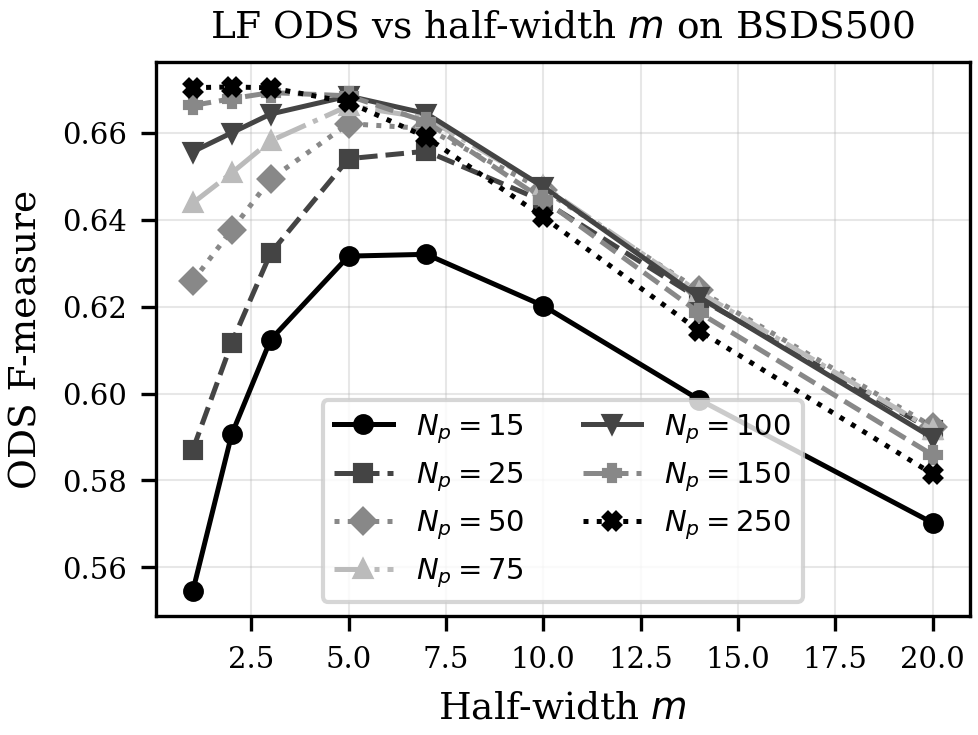
\includegraphics[width=\textwidth]{figures/fig_lf_ods_vs_m.png}
    \end{column}
  \end{columns}
\end{frame}

% ============================================================
\sectionsubtitle{WVF vs. classical operators and deep learning}
\section{Benchmarking}

\begin{frame}{WVF Outperforms All 54 Classical Operators}
  \begin{columns}[T]
    \begin{column}{0.35\textwidth}
      On BIPED v1:
      \begin{itemize}
        \item Best WVF: \textbf{0.812}
        \item Best classical (Prewitt-5): 0.788
        \item Gap: +0.024 ODS (3.0\%)
      \end{itemize}

      \vspace{0.5em}
      WVF exceeds \textit{every} classical configuration tested, spanning Sobel, Prewitt, LoG, DoG, Kirsch, Frei-Chen, and Scharr.
    \end{column}
    \begin{column}{0.62\textwidth}
      
\includegraphics[width=\textwidth]{figures/fig_classical_ranking.png}
    \end{column}
  \end{columns}
\end{frame}

\begin{frame}{Classical Scale Sensitivity}
  \begin{columns}[T]
    \begin{column}{0.35\textwidth}
      Every classical operator family shows a clear optimal scale --- performance degrades sharply beyond it.

      \vspace{0.5em}
      Sobel-51 scores only 0.428 versus Sobel-7 at 0.776.

      \vspace{0.5em}
      WVF's polynomial fitting performs a form of \textit{adaptive scale selection}, explaining its advantage.
    \end{column}
    \begin{column}{0.62\textwidth}
      
\includegraphics[width=\textwidth]{figures/fig_classical_scale_trend.png}
    \end{column}
  \end{columns}
\end{frame}

\begin{frame}{Computational Cost: WVF Is the Fastest Method}
  \begin{columns}[T]
    \begin{column}{0.38\textwidth}
      \begin{table}
        \centering
        \begin{tabular}{lrl}
          \toprule
          \textbf{Method} & \textbf{Time} & \textbf{Rel.} \\
          \midrule
          WVF           & 0.036s & $1.0\times$ \\
          PiDiNet       & 0.119s & $3.3\times$ \\
          DexiNed       & 0.226s & $6.3\times$ \\
          NBED          & 0.253s & $7.1\times$ \\
          TEED          & 0.538s & $15.1\times$ \\
          DiffusionEdge & 15.22s & $427\times$ \\
          \bottomrule
        \end{tabular}
      \end{table}

      WVF achieves real-time processing at 30+ fps.
    \end{column}
    \begin{column}{0.59\textwidth}
      
\includegraphics[width=\textwidth]{figures/fig_compute_cost.png}
    \end{column}
  \end{columns}
\end{frame}

% ============================================================
\sectionsubtitle{WVF adapts; deep learning collapses}
\section{Noise Robustness}

\begin{frame}{Optimal $N_p$ Shifts Dramatically Under Noise}
  \begin{columns}[T]
    \begin{column}{0.38\textwidth}
      Under severe Gaussian noise (SNR = 0.3):
      \begin{itemize}
        \item Optimal $N_p$ shifts from $\sim$40 to $\sim$440
        \item A $\sim$10$\times$ increase in support size
        \item Partially vindicates Bagan's $N_p = 250$
      \end{itemize}

      \vspace{0.5em}
      However, $d = 2$ remains universally optimal --- $d = 4$ is suboptimal at every SNR level.
    \end{column}
    \begin{column}{0.59\textwidth}
      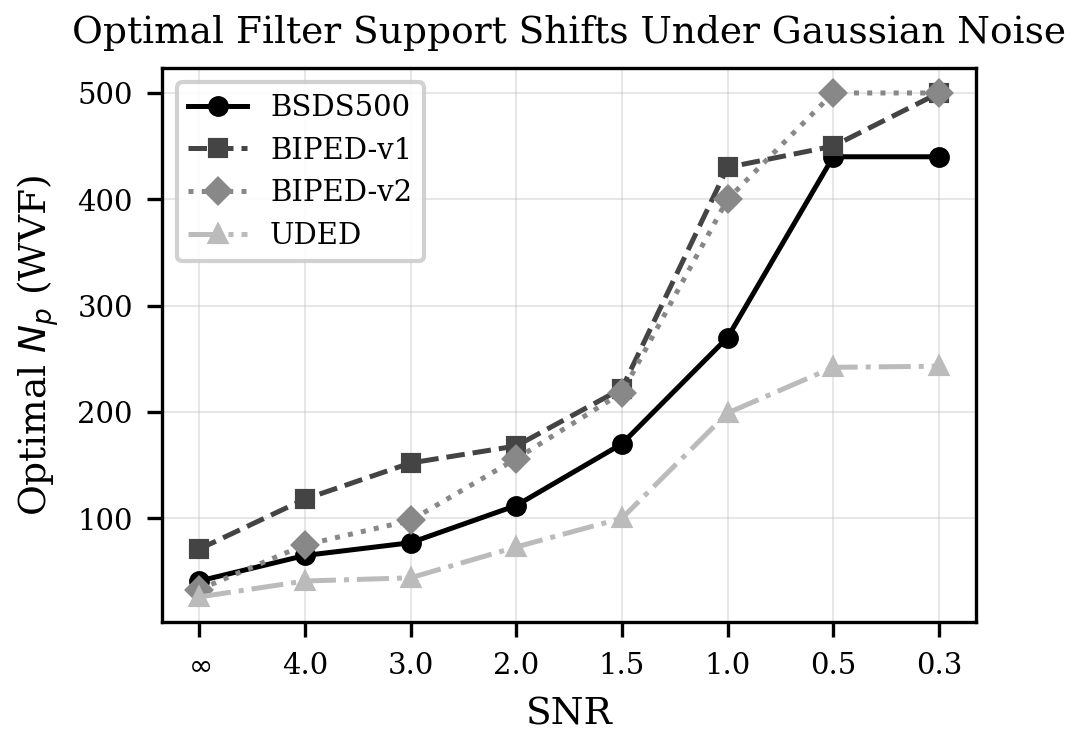
\includegraphics[width=\textwidth]{figures/fig_optimal_params_shift.png}
    \end{column}
  \end{columns}
\end{frame}

\begin{frame}{Noise-Type-Specific WVF Degradation}
  \begin{columns}[T]
    \begin{column}{0.38\textwidth}
      Degradation profiles vary by noise type:
      \begin{itemize}
        \item Speckle: least destructive (23\% drop)
        \item Poisson: intermediate (30\%)
        \item Salt-and-pepper: intermediate (31\%)
        \item Gaussian/uniform: most severe (36--37\%)
      \end{itemize}

      \vspace{0.5em}
      Ranking is consistent across all datasets.
    \end{column}
    \begin{column}{0.59\textwidth}
      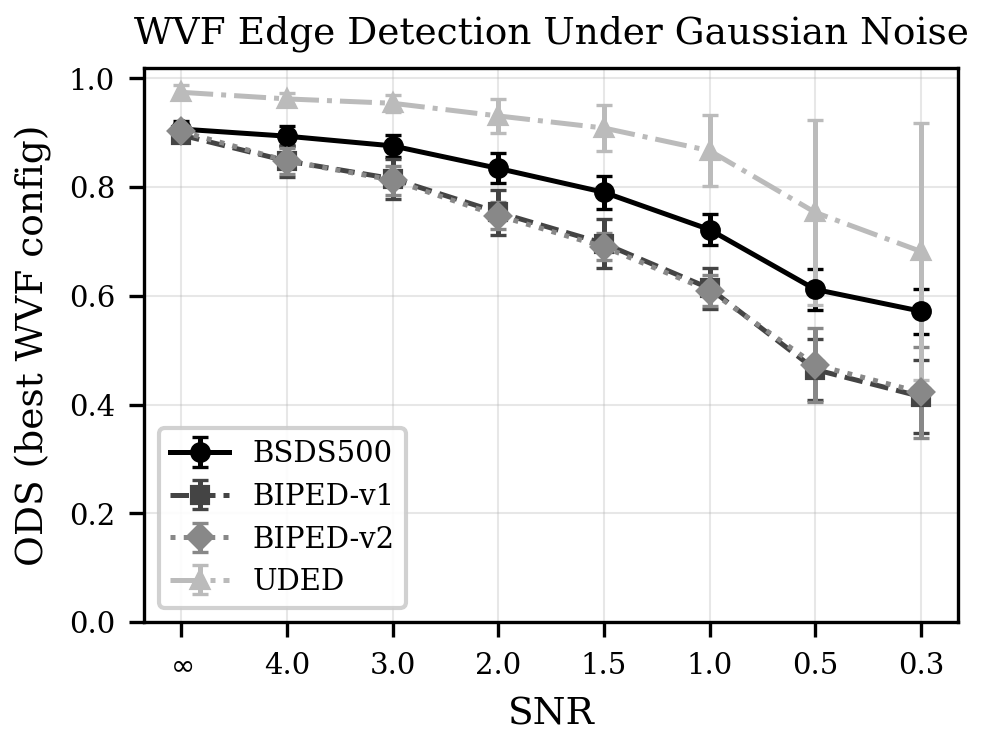
\includegraphics[width=\textwidth]{figures/fig_wvf_ods_vs_snr.png}
    \end{column}
  \end{columns}
\end{frame}

\begin{frame}{Deep Learning Models Collapse Under Noise}
  \begin{columns}[T]
    \begin{column}{0.38\textwidth}
      All 5 DL models degrade severely:
      \begin{itemize}
        \item PiDiNet: 0.876 $\to$ 0.329 (62\% loss)
        \item DexiNed: near-total collapse
        \item TEED: severe degradation
        \item NBED: most graceful decline
        \item DiffusionEdge: erratic behavior
      \end{itemize}

      \vspace{0.5em}
      None include noise augmentation in training.
    \end{column}
    \begin{column}{0.59\textwidth}
      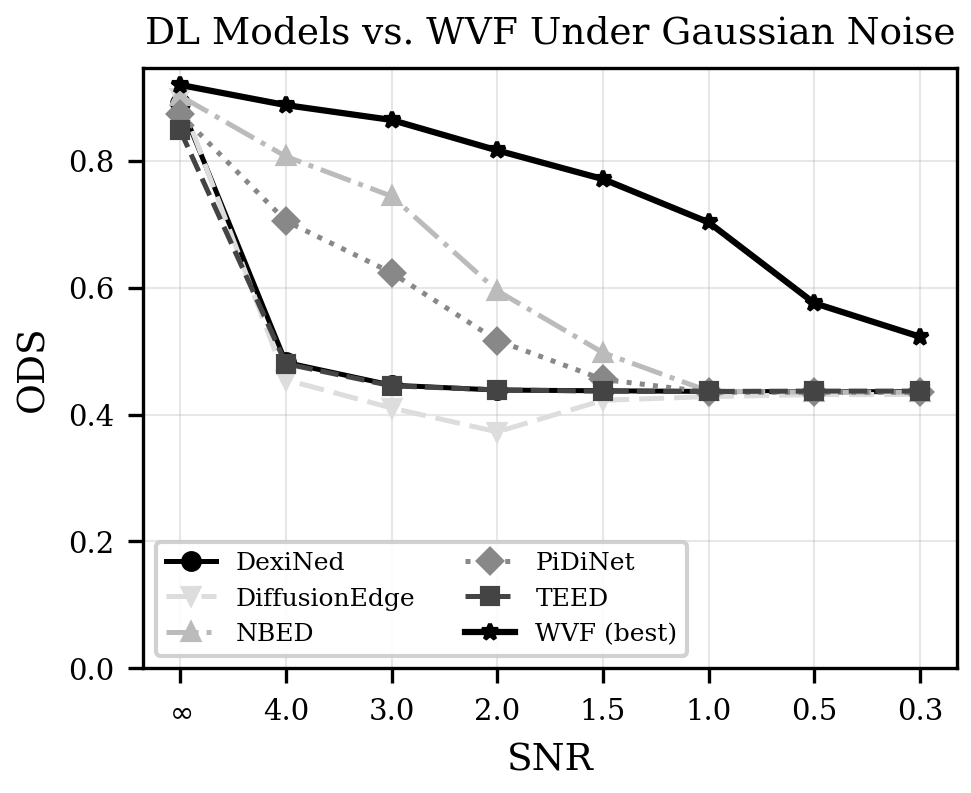
\includegraphics[width=\textwidth]{figures/fig_dl_degradation.png}
    \end{column}
  \end{columns}
\end{frame}

\begin{frame}{WVF Overtakes DL at Surprisingly Mild Noise}
  \begin{columns}[T]
    \begin{column}{0.38\textwidth}
      Crossover analysis:
      \begin{itemize}
        \item DexiNed, TEED: overtaken at \textit{all} SNR levels
        \item PiDiNet: overtaken at SNR $\approx$ 4.0
        \item NBED: most competitive, still exceeded
      \end{itemize}

      \vspace{0.5em}
      At SNR = 0.3: WVF beats \textit{every} DL model on \textit{every} test image (100\% crossover).
    \end{column}
    \begin{column}{0.59\textwidth}
      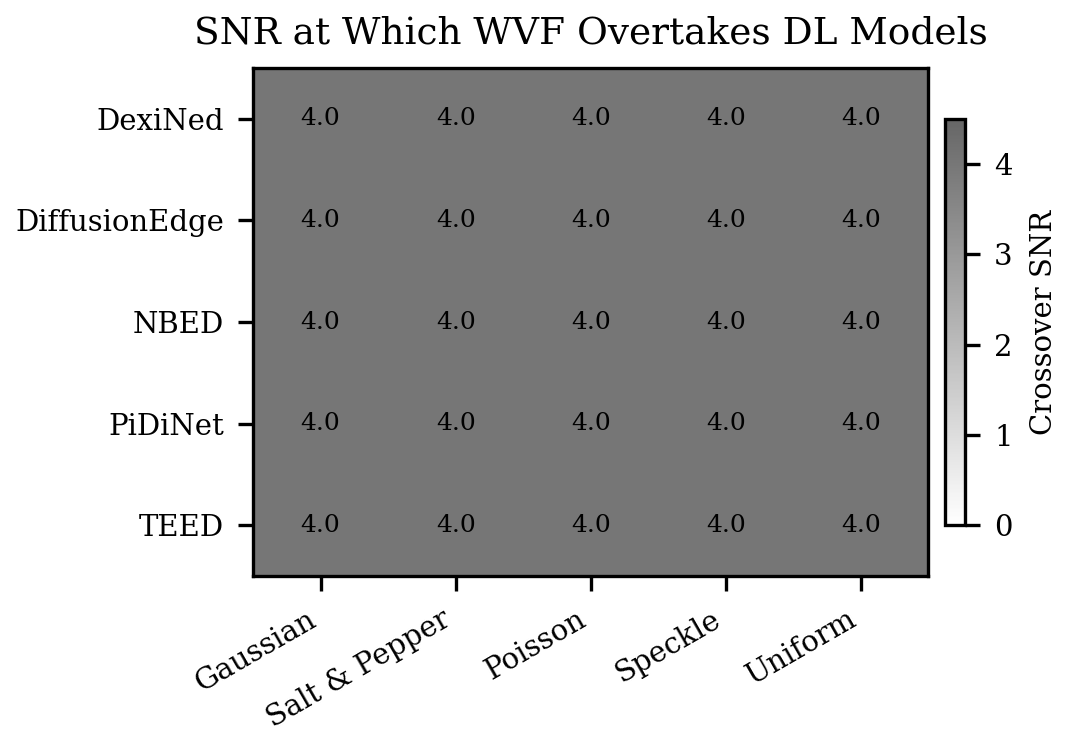
\includegraphics[width=\textwidth]{figures/fig_crossover_by_noise_type.png}
    \end{column}
  \end{columns}
\end{frame}

\begin{frame}{WVF vs. LF Under Noise}
  \begin{columns}[T]
    \begin{column}{0.38\textwidth}
      On clean data, WVF leads by $\sim$0.007 ODS.

      \vspace{0.5em}
      Under severe noise (SNR $\leq$ 1.0), the gap closes and LF slightly overtakes WVF for Gaussian, salt-and-pepper, and uniform noise.

      \vspace{0.5em}
      The reversal is modest (0.002--0.009 ODS) --- the LF's line-averaging provides marginal noise resilience.
    \end{column}
    \begin{column}{0.59\textwidth}
      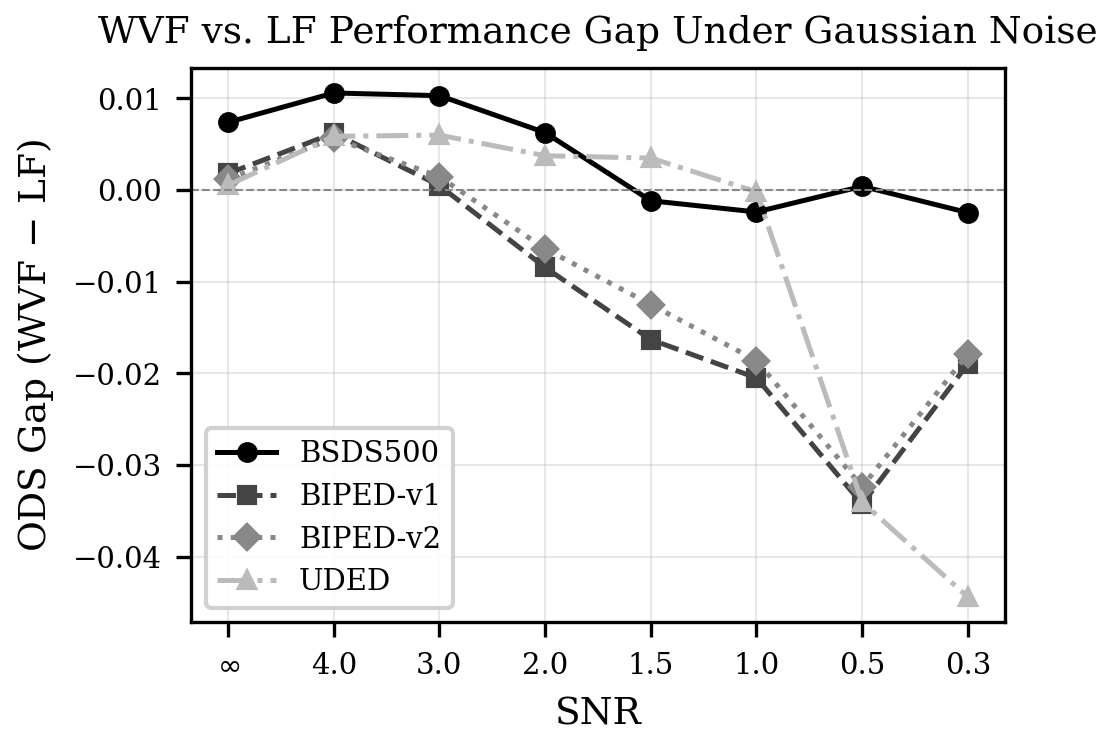
\includegraphics[width=\textwidth]{figures/fig_lf_vs_wvf_noise.png}
    \end{column}
  \end{columns}
\end{frame}

% ============================================================
\sectionsubtitle{Nonparametric tests confirm all major claims}
\section{Statistical Validation}

\begin{frame}{Cross-Dataset Ranking Consistency}
  \begin{columns}[T]
    \begin{column}{0.38\textwidth}
      Kendall's $W = 0.647$ (moderate concordance).

      \vspace{0.5em}
      UDED, BIPED v1, BIPED v2: $\rho > 0.96$ (near-perfect agreement).

      \vspace{0.5em}
      BSDS500 is a strong outlier: $\rho = 0.03$--$0.17$ with all other datasets.

      \vspace{0.5em}
      Top-10 configurations on BSDS500 share \textit{zero overlap} with other datasets.
    \end{column}
    \begin{column}{0.59\textwidth}
      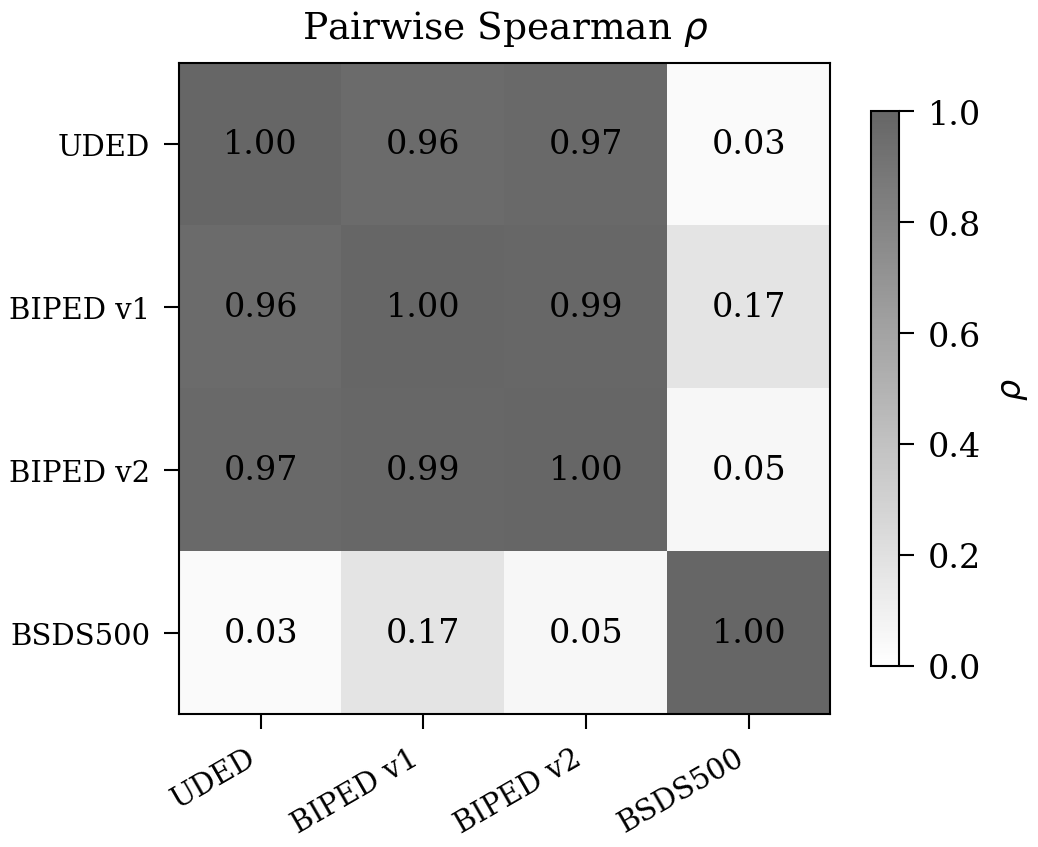
\includegraphics[width=\textwidth]{figures/fig_spearman_heatmap.png}
    \end{column}
  \end{columns}
\end{frame}

\begin{frame}{Parameter Sensitivity Analysis}
  \begin{columns}[T]
    \begin{column}{0.38\textwidth}
      Kruskal--Wallis analysis reveals parameter priority:

      \vspace{0.5em}
      \begin{table}
        \centering
        \begin{tabular}{lc}
          \toprule
          \textbf{Parameter} & $\eta^2$ \\
          \midrule
          $m$ (LF half-width) & 0.343 \\
          $N_p$ (support size) & $\sim$0.05 \\
          $N_s$ (orientations) & $\sim$0.05 \\
          $d$ (poly. degree)   & $<$0.01 \\
          \bottomrule
        \end{tabular}
      \end{table}

      \vspace{0.3em}
      $m$ is by far the most influential --- the LF's line extension is its biggest liability on clean data.
    \end{column}
    \begin{column}{0.59\textwidth}
      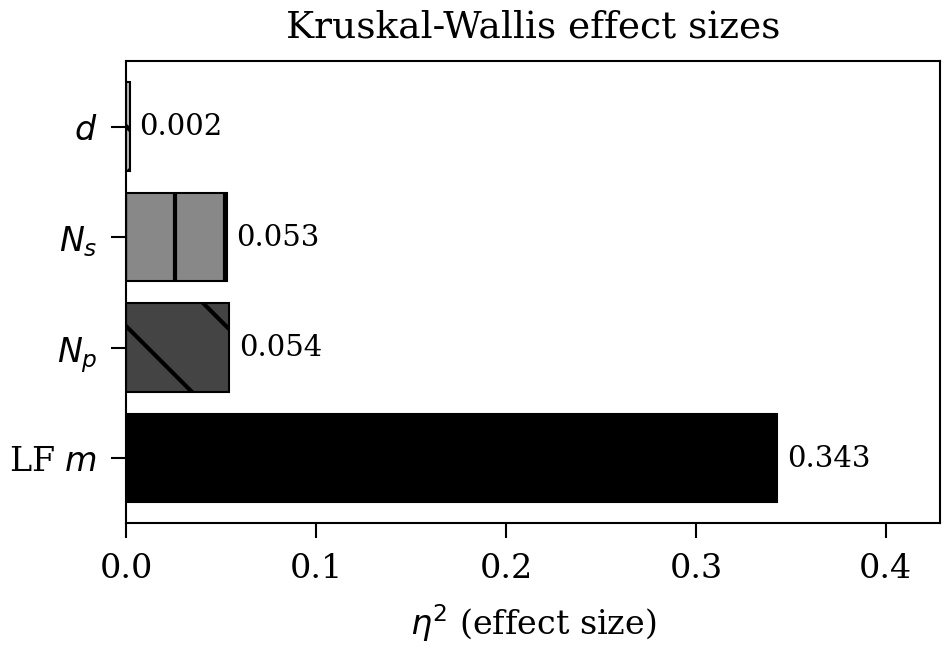
\includegraphics[width=\textwidth]{figures/fig_parameter_sensitivity.png}
    \end{column}
  \end{columns}
\end{frame}

% ============================================================
\sectionsubtitle{}
\section{Conclusion}

\begin{frame}{Six Definitive Findings}
  \begin{enumerate}
    \item \textbf{Published parameters are suboptimal}: $N_p = 25$--$100$, $d = 2$, $N_s = 4$ improves ODS by 0.01--0.16 with $112\times$ computational savings
    \item \textbf{WVF beats all 54 classical operators} by +2.4 ODS points
    \item \textbf{WVF is $3.3\times$--$427\times$ faster} than every DL model tested
    \item \textbf{Under noise, optimal $N_p$ shifts to 250--500}, partially vindicating Bagan and Wang's design
    \item \textbf{WVF overtakes DL models at mild noise} (SNR $\approx$ 4.0); 100\% crossover by SNR = 0.3
    \item \textbf{BSDS500 is a statistical outlier}: its rankings are uninformative about other domains ($\rho = 0.03$--$0.17$)
  \end{enumerate}
\end{frame}

\begin{frame}{Practical Recommendations}
  \begin{columns}[T]
    \begin{column}{0.48\textwidth}
      \textbf{Clean imagery}
      \begin{itemize}
        \item Use WVF (not LF)
        \item $N_p = 25$--$50$ (high-res) or $50$--$100$ (low-res)
        \item $d = 2$, $N_s = 4$
        \item Skip NMS (raw gradient maps score higher)
      \end{itemize}
    \end{column}
    \begin{column}{0.48\textwidth}
      \textbf{Noisy environments}
      \begin{itemize}
        \item Increase $N_p$ proportionally to noise level
        \item Moderate noise: $N_p = 65$--$112$
        \item Severe noise: $N_p = 250$--$500$
        \item $d = 2$ remains optimal at all SNR levels
      \end{itemize}
    \end{column}
  \end{columns}

  \vspace{1em}
  Edge detection method selection is fundamentally \textbf{condition-dependent}. WVF's principal strength is \textit{parametric adaptability} across the full spectrum of operating conditions.
\end{frame}

% ------ Thank You / Q&A ------
{
  \setbeamertemplate{footline}{}
  \begin{frame}[plain]
    \begin{tikzpicture}[remember picture, overlay]
      \fill[UofSCGarnet] (current page.south west) rectangle (current page.north east);
      \fill[UofSCDarkGarnet] (current page.south west) rectangle ([yshift=0.8cm]current page.south east);
      \draw[white, line width=0.5pt] ([yshift=0.8cm]current page.south west) -- ([yshift=0.8cm]current page.south east);
    \end{tikzpicture}
    \vfill
    \centering
    {\fontsize{50}{55}\selectfont\impactfont\color{UofSCWhite} THANK YOU!}\\[1em]
    {\Large\color{UofSCWhite} Questions \& Discussion}\\[0.5em]
    {\normalsize\color{UofSCGray30} jvaught@sc.edu}
    \vfill
  \end{frame}
}

\end{document}
